\pagestyle{plain}
\pagenumbering{arabic}
\chapter{Introduzione}
Il seguente testo si propone come relazione relativa all'esercitazione di \emph{Sicurezza Strutturale} del Corso di Laurea Magistrale in Ingegneria Civile. Nelle seguenti righe si riportano stralci del testo della suddetta esercitazione, con lo scopo di descrivere l'edificio oggetto d'esame.

\section{Descrizione dell'edificio}\label{sec:descrizioneEdificio}
L'edificio in esame ha una struttura multipiano, portante, in cemento armato. Il fabbricato è composto da un interrato (garage), un piano terra adibito a negozi, un \emph{piano primo} in cui sono presenti \emph{uffici aperti al pubblico}, mentre il piano superiore è destinato ad uso civile residenziale. Il solaio di copertura è piano, non praticabile, accessibile perciò solo dal personale addetto alla manutenzione.

Il complesso si trova in provincia di Trento ad altitudine pari alle ultime tre cifre del numero di matricola dello studente; considerando che al momento della redazione del seguente testo lo studente non è provvisto di un numero di matricola relativo al corso di laurea magistrale, i calcoli verranno eseguiti secondo la matricola del corso di laurea triennale. Ne consegue che, l'altitudine di riferimento relativa al livello medio dei mari è di
\begin{equation*}
 788\,m
\end{equation*}


Per l'analisi dei carichi gravanti, vengono riportate le stratigrafie dei principali solai e i pesi specifici dei vari materiali impiegati:
\begin{itemize}
 \item il solaio tra piano interrato e piano terra e il solaio di copertura sono realizzati con laste tralicciate di tipo Predalle di spessore $(4+16+5)\,\si{cm}$. Il peso strutturale del solaio è di $3.60\,\si{kN}/_{\si{m^2}}$;
 \item i \emph{solai tra piani intermedi} sono realizzati con travetti tralicciati in \emph{laterocemento} con spessore $(20+5)\,\si{cm}$. Il peso del solaio ultimato è di
 \begin{equation*}
  g_{1k_{solaio}} = 3.20\,\dfrac{kN}{m^2}
 \end{equation*}
 \item i \emph{solai interni} sono finiti all'\emph{estradosso} con un sottofondo di \emph{cls alleggerito} di spessore pari a $8\,\si{cm}$ e peso specifico $16\,kN/_{m^3}$, un \emph{massetto di allettamento} di $6\,\si{cm}$ e peso specifico $24\,kN/_{m^3}$ e infine un \emph{pavimento in ceramica} del peso di $0.50\,kN/_{m^2}$. All'\emph{intradosso} è presente $1\,\si{cm}$ di intonaco di peso specifico $20\,kN/_{m^3}$;
 \item il solaio di copertura è finito all'estradosso con uno strato isolante di spessore $20\,cm$ (peso specifico $0.30\,kN/_{m^3}$), un massetto in calcestruzzo alleggerito di spessore medio pari a $6\,cm$ (peso specifico $18\,kN/_{m^3}$), uno strato di impermeabilizzante di peso trascurabile e uno strato di ghiaino di $10\,cm$ (peso specifico $15\,kN/_{m^3}$). All'intradosso è finito con un centimetro di intonaco;
 \item i \emph{solai delle terrazze} presenti al piano primo sono finiti all'\emph{estradosso} con uno strato \emph{isolante} di $15\,\si{cm}$ e peso specifico $0.50\,kN/_{m^3}$, uno strato di impermeabilizzante di peso trascurabile, un \emph{massetto} in calcestruzzo di spessore medio pari a $6\,\si{cm}$ e peso specifico $24\,kN/_{m^3}$ e un \emph{pavimento} di peso $0.50\,kN/_{m^2}$. Il solaio è finito all'\emph{intradosso} con intonaco di spessore $1\,\si{cm}$;
 \item i \emph{tamponamenti perimetrali} sono realizzati in muratura di laterizio di spessore $30\,\si{cm}$ e peso specifico apparente pari a $10\,kN/_{m^3}$, \emph{cappotto esterno} di spessore $12\,\si{cm}$ (peso specifico $0.20\,kN/_{m^3}$) e all'interno $1\,\si{cm}$ di \emph{intonaco} (vedi caratteristiche sopra).
\end{itemize}


\section{Caratteristiche geometriche}\label{sec:geomCar}
Di seguito sono descritte le caratteristiche geometriche relative agli elementi strutturali in studio. In particolare, sono presenti:
\begin{itemize}
 \item pilastri a sezione quadrata di dimensioni $30 \times 30\,\si{cm}$;
 \item travi in spessore di solaio con larghezza pari a $60\,\si{cm}$;
 \item travi perimetrali di larghezza $30\,\si{cm}$ e altezza $50\,\si{cm}$;
 \item setti di spessore $30\,\si{cm}$.
\end{itemize}

Con riferimento a quanto descritto sopra, si allegano gli elaborati grafici forniti nel testo dell'esercitazione, in modo tale da avere un quadro generale del problema.
\cleardoublepage
\pagestyle{empty}{

\includepdf[pages=2,pagecommand={}, angle=90, width=\textwidth]{../Esercitazione_01}

\includepdf[pages=3,pagecommand={}, angle=90, width=\textwidth]{../Esercitazione_01}

\includepdf[pages=4,pagecommand={}, angle=90, width=\textwidth]{../Esercitazione_01}

\includepdf[pages=5,pagecommand={}, angle=90, width=\textwidth]{../Esercitazione_01}

\includepdf[pages=6,pagecommand={}, angle=90, width=\textwidth]{../Esercitazione_01}
}
\cleardoublepage
\pagestyle{plain}
Secondo le indicazioni riportate nel testo, con riferimento all'inziale del cognome dello studente, in questo documento si tratterà la trave al \emph{piano primo} da $P13 \div P18$ al \emph{vano scala}, e i pilastri $P27$ e $P36$ come segnati in figura~\ref{fig:pianoPrimo}.
\begin{figure}
 \centering
 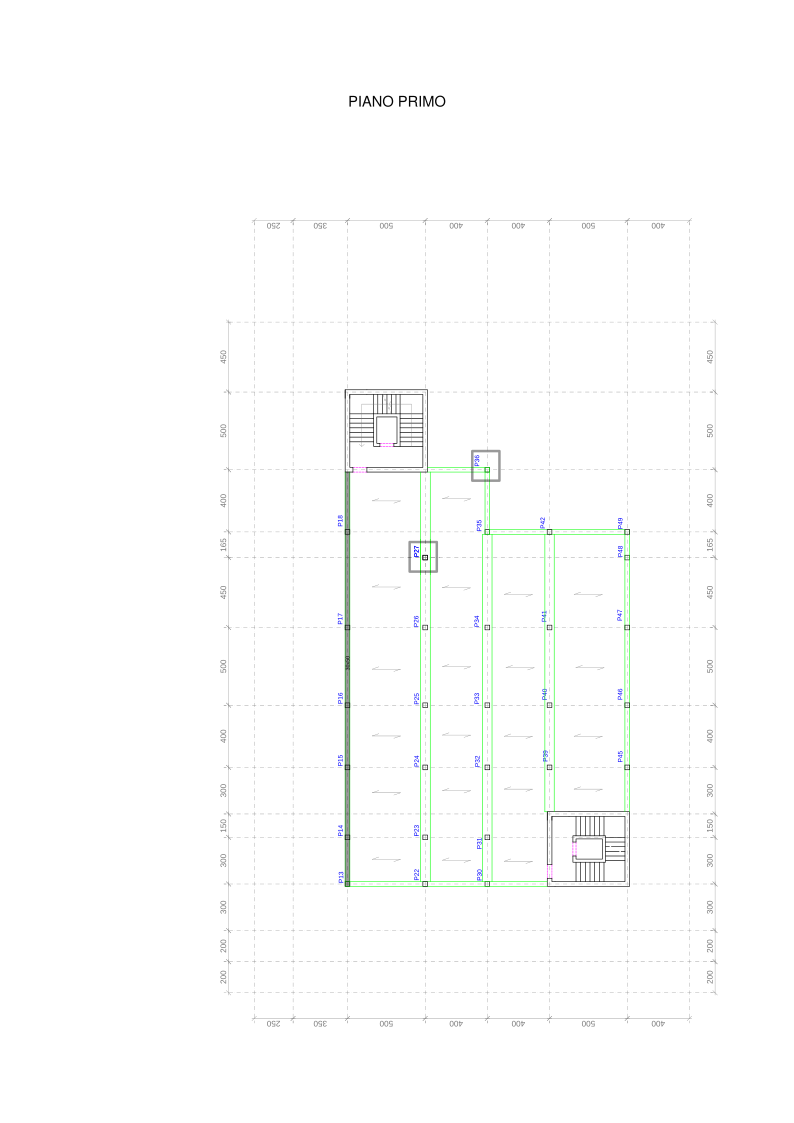
\includegraphics[height=.6\textheight]{../../pianoPrimo_esercitazione.png}
 \caption{Elementi strutturali in esame per il \emph{gruppo 2}}
 \label{fig:pianoPrimo}
\end{figure}

